% Options for packages loaded elsewhere
\PassOptionsToPackage{unicode}{hyperref}
\PassOptionsToPackage{hyphens}{url}
\PassOptionsToPackage{dvipsnames,svgnames*,x11names*}{xcolor}
%
\documentclass[
  10pt,
  ignorenonframetext,
]{beamer}
\usepackage{pgfpages}
\setbeamertemplate{caption}[numbered]
\setbeamertemplate{caption label separator}{: }
\setbeamercolor{caption name}{fg=normal text.fg}
\beamertemplatenavigationsymbolsempty
% Prevent slide breaks in the middle of a paragraph
\widowpenalties 1 10000
\raggedbottom
\setbeamertemplate{part page}{
  \centering
  \begin{beamercolorbox}[sep=16pt,center]{part title}
    \usebeamerfont{part title}\insertpart\par
  \end{beamercolorbox}
}
\setbeamertemplate{section page}{
  \centering
  \begin{beamercolorbox}[sep=12pt,center]{part title}
    \usebeamerfont{section title}\insertsection\par
  \end{beamercolorbox}
}
\setbeamertemplate{subsection page}{
  \centering
  \begin{beamercolorbox}[sep=8pt,center]{part title}
    \usebeamerfont{subsection title}\insertsubsection\par
  \end{beamercolorbox}
}
\AtBeginPart{
  \frame{\partpage}
}
\AtBeginSection{
  \ifbibliography
  \else
    \frame{\sectionpage}
  \fi
}
\AtBeginSubsection{
  \frame{\subsectionpage}
}
\usepackage{lmodern}
\usepackage{amsmath}
\usepackage{ifxetex,ifluatex}
\ifnum 0\ifxetex 1\fi\ifluatex 1\fi=0 % if pdftex
  \usepackage[T1]{fontenc}
  \usepackage[utf8]{inputenc}
  \usepackage{textcomp} % provide euro and other symbols
  \usepackage{amssymb}
\else % if luatex or xetex
  \usepackage{unicode-math}
  \defaultfontfeatures{Scale=MatchLowercase}
  \defaultfontfeatures[\rmfamily]{Ligatures=TeX,Scale=1}
\fi
\usetheme[]{metropolis}
% Use upquote if available, for straight quotes in verbatim environments
\IfFileExists{upquote.sty}{\usepackage{upquote}}{}
\IfFileExists{microtype.sty}{% use microtype if available
  \usepackage[]{microtype}
  \UseMicrotypeSet[protrusion]{basicmath} % disable protrusion for tt fonts
}{}
\makeatletter
\@ifundefined{KOMAClassName}{% if non-KOMA class
  \IfFileExists{parskip.sty}{%
    \usepackage{parskip}
  }{% else
    \setlength{\parindent}{0pt}
    \setlength{\parskip}{6pt plus 2pt minus 1pt}}
}{% if KOMA class
  \KOMAoptions{parskip=half}}
\makeatother
\usepackage{xcolor}
\IfFileExists{xurl.sty}{\usepackage{xurl}}{} % add URL line breaks if available
\IfFileExists{bookmark.sty}{\usepackage{bookmark}}{\usepackage{hyperref}}
\hypersetup{
  pdftitle={A minimal example},
  pdfauthor={Reproducible Researcher},
  colorlinks=true,
  linkcolor=teal,
  filecolor=Maroon,
  citecolor=Blue,
  urlcolor=teal,
  pdfcreator={LaTeX via pandoc}}
\urlstyle{same} % disable monospaced font for URLs
\newif\ifbibliography
\usepackage{color}
\usepackage{fancyvrb}
\newcommand{\VerbBar}{|}
\newcommand{\VERB}{\Verb[commandchars=\\\{\}]}
\DefineVerbatimEnvironment{Highlighting}{Verbatim}{commandchars=\\\{\}}
% Add ',fontsize=\small' for more characters per line
\usepackage{framed}
\definecolor{shadecolor}{RGB}{248,248,248}
\newenvironment{Shaded}{\begin{snugshade}}{\end{snugshade}}
\newcommand{\AlertTok}[1]{\textcolor[rgb]{0.94,0.16,0.16}{#1}}
\newcommand{\AnnotationTok}[1]{\textcolor[rgb]{0.56,0.35,0.01}{\textbf{\textit{#1}}}}
\newcommand{\AttributeTok}[1]{\textcolor[rgb]{0.77,0.63,0.00}{#1}}
\newcommand{\BaseNTok}[1]{\textcolor[rgb]{0.00,0.00,0.81}{#1}}
\newcommand{\BuiltInTok}[1]{#1}
\newcommand{\CharTok}[1]{\textcolor[rgb]{0.31,0.60,0.02}{#1}}
\newcommand{\CommentTok}[1]{\textcolor[rgb]{0.56,0.35,0.01}{\textit{#1}}}
\newcommand{\CommentVarTok}[1]{\textcolor[rgb]{0.56,0.35,0.01}{\textbf{\textit{#1}}}}
\newcommand{\ConstantTok}[1]{\textcolor[rgb]{0.00,0.00,0.00}{#1}}
\newcommand{\ControlFlowTok}[1]{\textcolor[rgb]{0.13,0.29,0.53}{\textbf{#1}}}
\newcommand{\DataTypeTok}[1]{\textcolor[rgb]{0.13,0.29,0.53}{#1}}
\newcommand{\DecValTok}[1]{\textcolor[rgb]{0.00,0.00,0.81}{#1}}
\newcommand{\DocumentationTok}[1]{\textcolor[rgb]{0.56,0.35,0.01}{\textbf{\textit{#1}}}}
\newcommand{\ErrorTok}[1]{\textcolor[rgb]{0.64,0.00,0.00}{\textbf{#1}}}
\newcommand{\ExtensionTok}[1]{#1}
\newcommand{\FloatTok}[1]{\textcolor[rgb]{0.00,0.00,0.81}{#1}}
\newcommand{\FunctionTok}[1]{\textcolor[rgb]{0.00,0.00,0.00}{#1}}
\newcommand{\ImportTok}[1]{#1}
\newcommand{\InformationTok}[1]{\textcolor[rgb]{0.56,0.35,0.01}{\textbf{\textit{#1}}}}
\newcommand{\KeywordTok}[1]{\textcolor[rgb]{0.13,0.29,0.53}{\textbf{#1}}}
\newcommand{\NormalTok}[1]{#1}
\newcommand{\OperatorTok}[1]{\textcolor[rgb]{0.81,0.36,0.00}{\textbf{#1}}}
\newcommand{\OtherTok}[1]{\textcolor[rgb]{0.56,0.35,0.01}{#1}}
\newcommand{\PreprocessorTok}[1]{\textcolor[rgb]{0.56,0.35,0.01}{\textit{#1}}}
\newcommand{\RegionMarkerTok}[1]{#1}
\newcommand{\SpecialCharTok}[1]{\textcolor[rgb]{0.00,0.00,0.00}{#1}}
\newcommand{\SpecialStringTok}[1]{\textcolor[rgb]{0.31,0.60,0.02}{#1}}
\newcommand{\StringTok}[1]{\textcolor[rgb]{0.31,0.60,0.02}{#1}}
\newcommand{\VariableTok}[1]{\textcolor[rgb]{0.00,0.00,0.00}{#1}}
\newcommand{\VerbatimStringTok}[1]{\textcolor[rgb]{0.31,0.60,0.02}{#1}}
\newcommand{\WarningTok}[1]{\textcolor[rgb]{0.56,0.35,0.01}{\textbf{\textit{#1}}}}
\usepackage{longtable,booktabs}
\usepackage{caption}
% Make caption package work with longtable
\makeatletter
\def\fnum@table{\tablename~\thetable}
\makeatother
\setlength{\emergencystretch}{3em} % prevent overfull lines
\providecommand{\tightlist}{%
  \setlength{\itemsep}{0pt}\setlength{\parskip}{0pt}}
\setcounter{secnumdepth}{-\maxdimen} % remove section numbering
\ifluatex
  \usepackage{selnolig}  % disable illegal ligatures
\fi

\title{A minimal example}
\author{Reproducible Researcher}
\date{2020-11-13}
\institute{University of Minho}

\begin{document}
\frame{\titlepage}

\begin{frame}[allowframebreaks]
  \tableofcontents[hideallsubsections]
\end{frame}
\hypertarget{the-basics}{%
\section{The Basics}\label{the-basics}}

\begin{frame}[fragile]{Basic set-up of a Rmd beamer presentation}
\protect\hypertarget{basic-set-up-of-a-rmd-beamer-presentation}{}
\begin{itemize}[<+->]
\tightlist
\item
  in our YAML header, we have specified the option
  \texttt{slide\_level:2}
\item
  \rightarrow we start a new slide after each
  \textbf{\texttt{\#\#\ Section\ Level\ 2\ Heading}}
\end{itemize}

\pause

\begin{verbatim}
---
output: 
  beamer_presentation: 
    slide_level: 2
---    
\end{verbatim}

\pause

\begin{itemize}[<+->]
\tightlist
\item
  each \textbf{\texttt{\#\ Section\ Level\ 1\ Heading}} inserts a new
  section slide
\item
  for a detailed overview of the beamer template used by Pandoc, please
  consult \href{}{}.
\item
  you can also load your own beamer template by specifying the argument
  \texttt{template:\ minho\_university.tex}
\end{itemize}
\end{frame}

\begin{frame}{Bullet points}
\protect\hypertarget{bullet-points}{}
\begin{itemize}[<+->]
\tightlist
\item
  Bullet 1
\item
  Bullet 2
\item
  Bullet 3

  \begin{itemize}[<+->]
  \tightlist
  \item
    subitem 1
  \item
    subitem 2
  \end{itemize}
\end{itemize}
\end{frame}

\begin{frame}[fragile]{Slide with actual R Output}
\protect\hypertarget{slide-with-actual-r-output}{}
\begin{itemize}[<+->]
\tightlist
\item
  specify \textbf{chunk option}: \texttt{echo=TRUE}
\end{itemize}

\begin{Shaded}
\begin{Highlighting}[]
\FunctionTok{head}\NormalTok{(penguins)}
\end{Highlighting}
\end{Shaded}

\begin{verbatim}
# A tibble: 6 x 8
  species island bill_length_mm bill_depth_mm flipper_length_~ body_mass_g sex  
  <fct>   <fct>           <dbl>         <dbl>            <int>       <int> <fct>
1 Adelie  Torge~           39.1          18.7              181        3750 male 
2 Adelie  Torge~           39.5          17.4              186        3800 fema~
3 Adelie  Torge~           40.3          18                195        3250 fema~
4 Adelie  Torge~           NA            NA                 NA          NA <NA> 
5 Adelie  Torge~           36.7          19.3              193        3450 fema~
6 Adelie  Torge~           39.3          20.6              190        3650 male 
# ... with 1 more variable: year <int>
\end{verbatim}
\end{frame}

\begin{frame}{Including Math}
\protect\hypertarget{including-math}{}
\begin{equation*}
    e = \lim_{n\to \infty} \left(1 + \frac{1}{n}\right)^n
\end{equation*}
\end{frame}

\begin{frame}[fragile]{Including images}
\protect\hypertarget{including-images}{}
\begin{itemize}[<+->]
\tightlist
\item
  Images can be useful for presentations:
\end{itemize}

\pause

\begin{figure}

{\centering 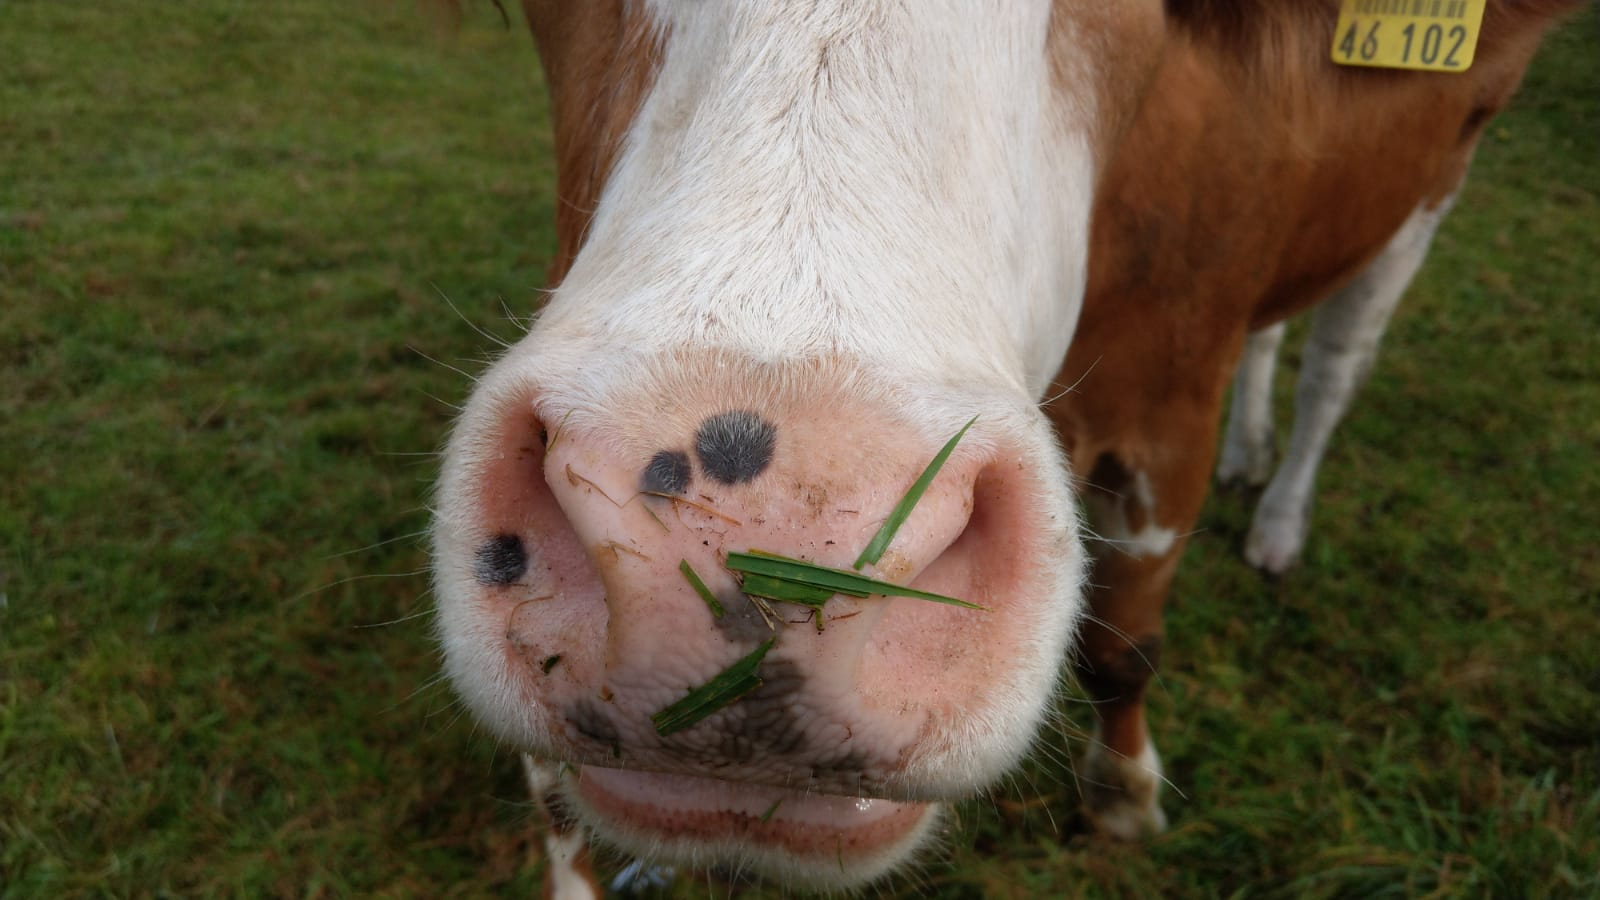
\includegraphics[width=0.4\linewidth]{figs/cow} 

}

\caption{A nice cow}\label{fig:unnamed-chunk-1}
\end{figure}

\pause

\begin{itemize}[<+->]
\tightlist
\item
  Global options for inclusion of figures in YAML header
\end{itemize}

\begin{verbatim}
---
output:
  pdf_document:
    fig_width: 7
    fig_height: 6
---
\end{verbatim}
\end{frame}

\hypertarget{integrating-content-and-code}{%
\section{Integrating content and
code}\label{integrating-content-and-code}}

\begin{frame}[fragile]{Including graphs - \texttt{ggplot}}
\protect\hypertarget{including-graphs---ggplot}{}
\begin{center}\includegraphics[width=1\linewidth]{figs/figggplot-1} \end{center}

\pause

\begin{itemize}[<+->]
\tightlist
\item
  \texttt{showtext} package: match fonts of presentation with the fonts
  in ggplot:
\item
  set chunk option to: \texttt{fig.showtext\ =\ TRUE}
\item
  \texttt{showtext\_auto()} before opening a new graphic device
\end{itemize}
\end{frame}

\begin{frame}[fragile]{Including tables - basic \texttt{kable}}
\protect\hypertarget{including-tables---basic-kable}{}
\begin{Shaded}
\begin{Highlighting}[]
\FunctionTok{kable}\NormalTok{(}
\NormalTok{  penguins }\SpecialCharTok{\%\textgreater{}\%}
    \FunctionTok{group\_by}\NormalTok{(species) }\SpecialCharTok{\%\textgreater{}\%}
    \CommentTok{\# calculate mean by species}
    \FunctionTok{summarize}\NormalTok{(}\FunctionTok{across}\NormalTok{(}
      \FunctionTok{where}\NormalTok{(is.numeric),}
      \SpecialCharTok{\textasciitilde{}} \FunctionTok{mean}\NormalTok{(., }\AttributeTok{na.rm =}\NormalTok{ T)}
\NormalTok{    )) }\SpecialCharTok{\%\textgreater{}\%}
    \CommentTok{\# drop the year variable for the printed table}
    \FunctionTok{select}\NormalTok{(}\SpecialCharTok{{-}}\NormalTok{year)}
\NormalTok{)}
\end{Highlighting}
\end{Shaded}

\begin{longtable}[]{@{}lrrrr@{}}
\toprule
species & bill\_length\_mm & bill\_depth\_mm & flipper\_length\_mm &
body\_mass\_g\tabularnewline
\midrule
\endhead
Adelie & 38.79139 & 18.34636 & 189.9536 & 3700.662\tabularnewline
Chinstrap & 48.83382 & 18.42059 & 195.8235 & 3733.088\tabularnewline
Gentoo & 47.50488 & 14.98211 & 217.1870 & 5076.016\tabularnewline
\bottomrule
\end{longtable}
\end{frame}

\begin{frame}[fragile]{Including tables - advanced styling with
\texttt{kable}}
\protect\hypertarget{including-tables---advanced-styling-with-kable}{}
\begin{itemize}[<+->]
\tightlist
\item
  use \texttt{kable} together with \texttt{kableExtra} for advanced
  styling options
\end{itemize}

\pause

\begin{table}[!h]

\caption{\label{tab:kable-advanced}Differences in Flipper and Bill Length across Penguin Species}
\centering
\resizebox{\linewidth}{!}{
\begin{tabular}[t]{lrrrr}
\toprule
Species & Bill Length
(mm) & Bill Depth
(mm) & Flipper Length
(mm) & Body Mass
(kg)\\
\midrule
Adelie & 38.79 & 18.35 & 189.95 & 3700.66\\
Chinstrap & 48.83 & 18.42 & 195.82 & 3733.09\\
Gentoo & 47.50 & 14.98 & 217.19 & 5076.02\\
\bottomrule
\end{tabular}}
\end{table}

\pause

\begin{itemize}[<+->]
\tightlist
\item
  find the full documentation of \texttt{kableExtra} for PDF documents
  \href{http://haozhu233.github.io/kableExtra/awesome_table_in_pdf.pdf}{here}
\end{itemize}
\end{frame}

\hypertarget{advanced-options-and-further-customization}{%
\section{Advanced options and further
customization}\label{advanced-options-and-further-customization}}

\begin{frame}{Tweaking and more advanced options}
\protect\hypertarget{tweaking-and-more-advanced-options}{}
\begin{itemize}[<+->]
\tightlist
\item
  long, extensive and \textbf{highly useful} documentation of the
  different \href{https://yihui.org/knitr/options/}{knitr chunk options}
\end{itemize}
\end{frame}

\end{document}
